\chapter{Resultados e Discussão}\label{cap:resultados}

Após entender o funcionamento dos algoritmos e definir a metodologia para análise, primeiramente foram executadas diversas iterações de classificação sobre o conjunto de imagens utilizando o método de Viola-Jones, variando os parâmetros de fator de escala (FE) para e número mínimo de vizinhos (MV), explicados na Seção \ref{sec:parametrizacao}, para que fosse identificada a melhor combinação de parâmetros para o objetivo atual.

Cada um dos resultados obtidos neste primeiro teste foi listado como um item da Tabela \ref{tab:results_identify}, onde lucro refere-se ao lucro obtido por imagem analisada e os resultados foram ordenados do mais lucrativo para o menos lucrativo.

Os resultados do teste com o método de Viola-Jones também foram exibidos no espaço ROC na Figura \ref{fig:results_roc} (foi utilizado um recorte apenas da parte superior para facilitar a visualização), destacando com cores os 3 cenários mais lucrativos, que também são identificados por letras correspondentes às exibidas na Tabela \ref{tab:results_identify}. Esse formato de exposição dos resultados torna facilita a comparação, e também se torna simples observar quais estão posicionado acima o limite lucrativo traçado.

\begin{figure}[htb]
    \centering
    \caption{Resultados dos testes do método de Viola-Jones exibidos sobre o espaço ROC.}
    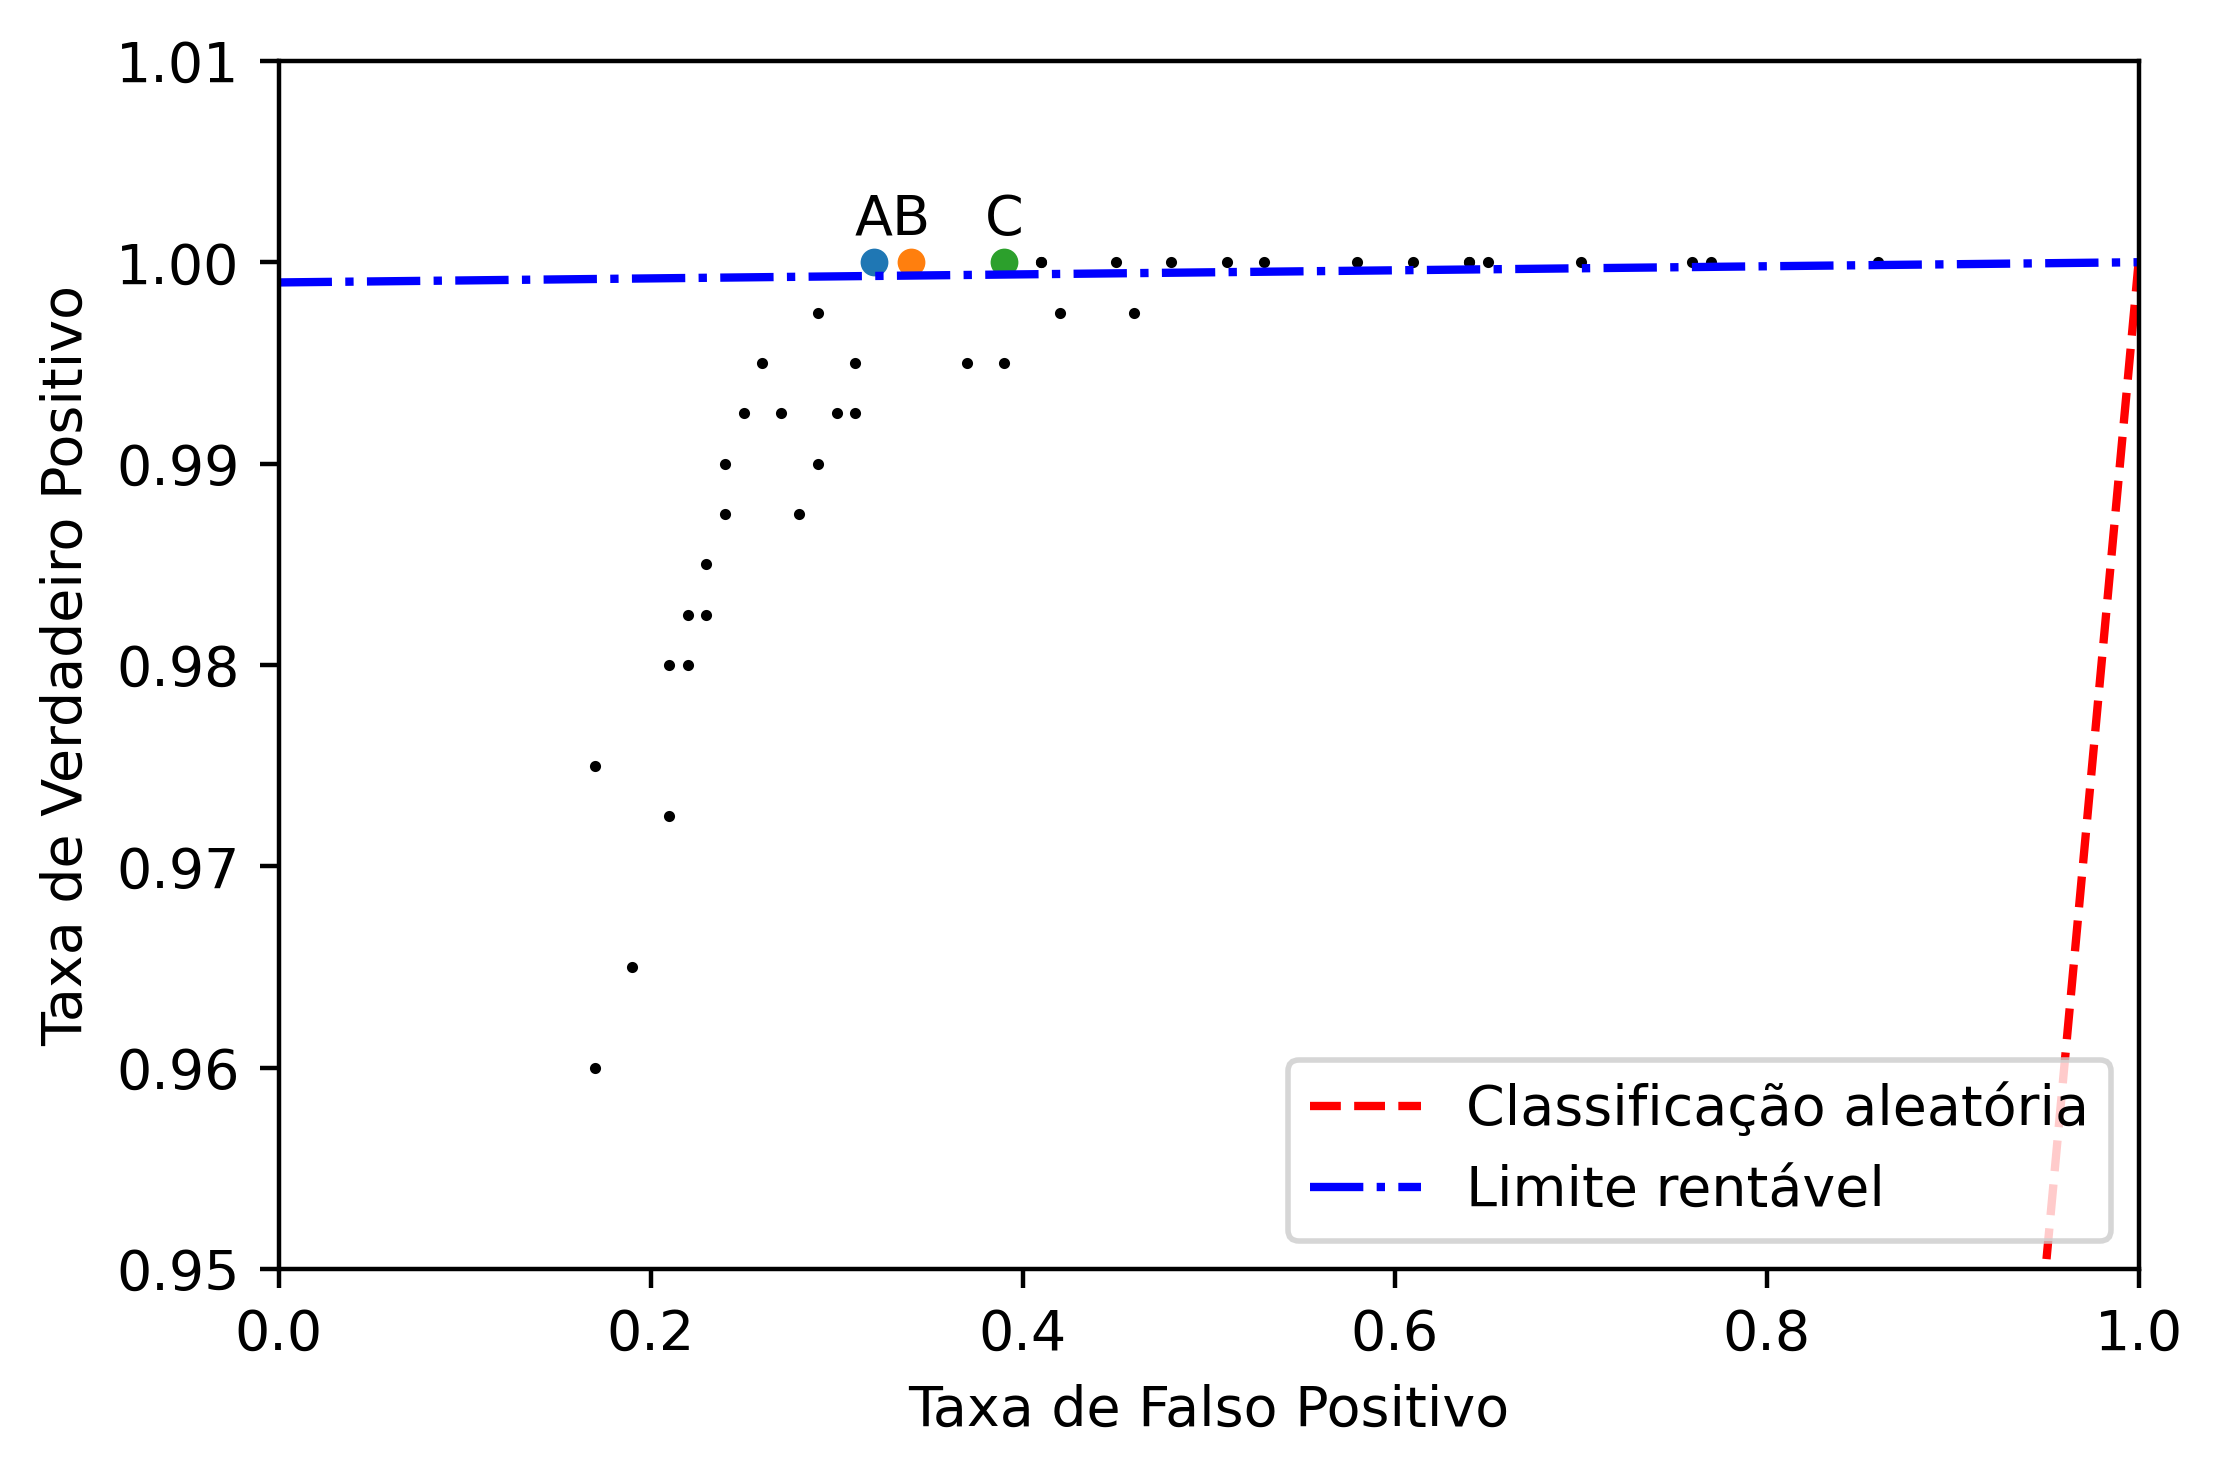
\includegraphics[scale=1]{figs/curva_roc_results_viola.png}
    \legend{Fonte: Própria (2020)}
    \label{fig:results_roc}
\end{figure}

\begin{table}[htbp]
    \caption{Resultados obtidos com o método de Viola-Jones.}
    \label{tab:results_identify}
    \centering
    \begin{tabular}{crrrrrr}
        \hline\hline
        Letra & FE   & MV & sensibilidade & Especificidade & Acurácia & Lucro$^1$  \\
        \hline
        A     & 1,10 & 4  & 100,00\%      & 68,00\%        & 93,60\%  & R\$ 0,136  \\
        B     & 1,30 & 1  & 100,00\%      & 66,00\%        & 93,20\%  & R\$ 0,132  \\
        C     & 1,10 & 3  & 100,00\%      & 61,00\%        & 92,20\%  & R\$ 0,122  \\
        -     & 1,25 & 1  & 100,00\%      & 59,00\%        & 91,80\%  & R\$ 0,118  \\
        -     & 1,05 & 5  & 100,00\%      & 59,00\%        & 91,80\%  & R\$ 0,118  \\
        -     & 1,05 & 4  & 100,00\%      & 55,00\%        & 91,00\%  & R\$ 0,110  \\
        -     & 1,10 & 2  & 100,00\%      & 52,00\%        & 90,40\%  & R\$ 0,104  \\
        -     & 1,15 & 1  & 100,00\%      & 49,00\%        & 89,80\%  & R\$ 0,098  \\
        -     & 1,05 & 3  & 100,00\%      & 47,00\%        & 89,40\%  & R\$ 0,094  \\
        -     & 1,10 & 1  & 100,00\%      & 42,00\%        & 88,40\%  & R\$ 0,084  \\
        -     & 1,05 & 2  & 100,00\%      & 39,00\%        & 87,80\%  & R\$ 0,078  \\
        -     & 1,30 & 0  & 100,00\%      & 36,00\%        & 87,20\%  & R\$ 0,072  \\
        -     & 1,25 & 0  & 100,00\%      & 36,00\%        & 87,20\%  & R\$ 0,072  \\
        -     & 1,20 & 0  & 100,00\%      & 35,00\%        & 87,00\%  & R\$ 0,070  \\
        -     & 1,05 & 1  & 100,00\%      & 30,00\%        & 86,00\%  & R\$ 0,060  \\
        -     & 1,15 & 0  & 100,00\%      & 24,00\%        & 84,80\%  & R\$ 0,048  \\
        -     & 1,10 & 0  & 100,00\%      & 23,00\%        & 84,60\%  & R\$ 0,046  \\
        -     & 1,05 & 0  & 100,00\%      & 14,00\%        & 82,80\%  & R\$ 0,028  \\
        -     & 1,10 & 5  & 99,75\%       & 71,00\%        & 94,00\%  & -R\$ 0,356 \\
        -     & 1,15 & 2  & 99,75\%       & 58,00\%        & 91,40\%  & -R\$ 0,382 \\
        -     & 1,20 & 1  & 99,75\%       & 54,00\%        & 90,60\%  & -R\$ 0,390 \\
        -     & 1,10 & 6  & 99,50\%       & 74,00\%        & 94,40\%  & -R\$ 0,848 \\
        -     & 1,20 & 2  & 99,50\%       & 69,00\%        & 93,40\%  & -R\$ 0,858 \\
        -     & 1,15 & 3  & 99,50\%       & 63,00\%        & 92,20\%  & -R\$ 0,870 \\
        -     & 1,05 & 6  & 99,50\%       & 61,00\%        & 91,80\%  & -R\$ 0,874 \\
        -     & 1,30 & 2  & 99,25\%       & 75,00\%        & 94,40\%  & -R\$ 1,344 \\
        -     & 1,15 & 5  & 99,25\%       & 73,00\%        & 94,00\%  & -R\$ 1,348 \\
        -     & 1,15 & 4  & 99,25\%       & 70,00\%        & 93,40\%  & -R\$ 1,354 \\
        -     & 1,25 & 2  & 99,25\%       & 69,00\%        & 93,20\%  & -R\$ 1,356 \\
        -     & 1,15 & 6  & 99,00\%       & 76,00\%        & 94,40\%  & -R\$ 1,840 \\
        -     & 1,20 & 3  & 99,00\%       & 71,00\%        & 93,40\%  & -R\$ 1,850 \\
        -     & 1,20 & 4  & 98,75\%       & 76,00\%        & 94,20\%  & -R\$ 2,338 \\
        -     & 1,25 & 3  & 98,75\%       & 72,00\%        & 93,40\%  & -R\$ 2,346 \\
        -     & 1,30 & 3  & 98,50\%       & 77,00\%        & 94,20\%  & -R\$ 2,834 \\
        -     & 1,20 & 5  & 98,25\%       & 78,00\%        & 94,20\%  & -R\$ 3,330 \\
        -     & 1,25 & 4  & 98,25\%       & 77,00\%        & 94,00\%  & -R\$ 3,332 \\
        -     & 1,25 & 5  & 98,00\%       & 79,00\%        & 94,20\%  & -R\$ 3,826 \\
        -     & 1,20 & 6  & 98,00\%       & 78,00\%        & 94,00\%  & -R\$ 3,828 \\
        -     & 1,25 & 6  & 97,50\%       & 83,00\%        & 94,60\%  & -R\$ 4,814 \\
        -     & 1,30 & 4  & 97,25\%       & 79,00\%        & 93,60\%  & -R\$ 5,320 \\
        -     & 1,30 & 5  & 96,50\%       & 81,00\%        & 93,40\%  & -R\$ 6,810 \\
        -     & 1,30 & 6  & 96,00\%       & 83,00\%        & 93,40\%  & -R\$ 7,802 \\
        \hline\hline
    \end{tabular}
\end{table}

É interessante ressaltar aqui que aproximadamente metade dos resultados apresentam lucro negativo, ou seja, prejuízo, mostrando a importância do ajuste correto dos parâmetros e também que nem sempre a aplicação do modelo é lucrativa para empresas.

Além dos testes com o método de Viola-Jones, também foi executado um teste utilizando o método MTCNN, este resultado foi exibido no espaço ROC na Figura \ref{fig:results_roc_mtcnn} e mais detalhadamente na Tabela \ref{tab:results_mtcnn}, juntamente com o melhor resultado obtido utilizando Viola-Jones, para que fosse feita a comparação.

\begin{figure}[htb]
    \centering
    \caption{Resultado do método MTCNN e melhor resultado do método de Viola-Jones exibidos sobre o espaço ROC.}
    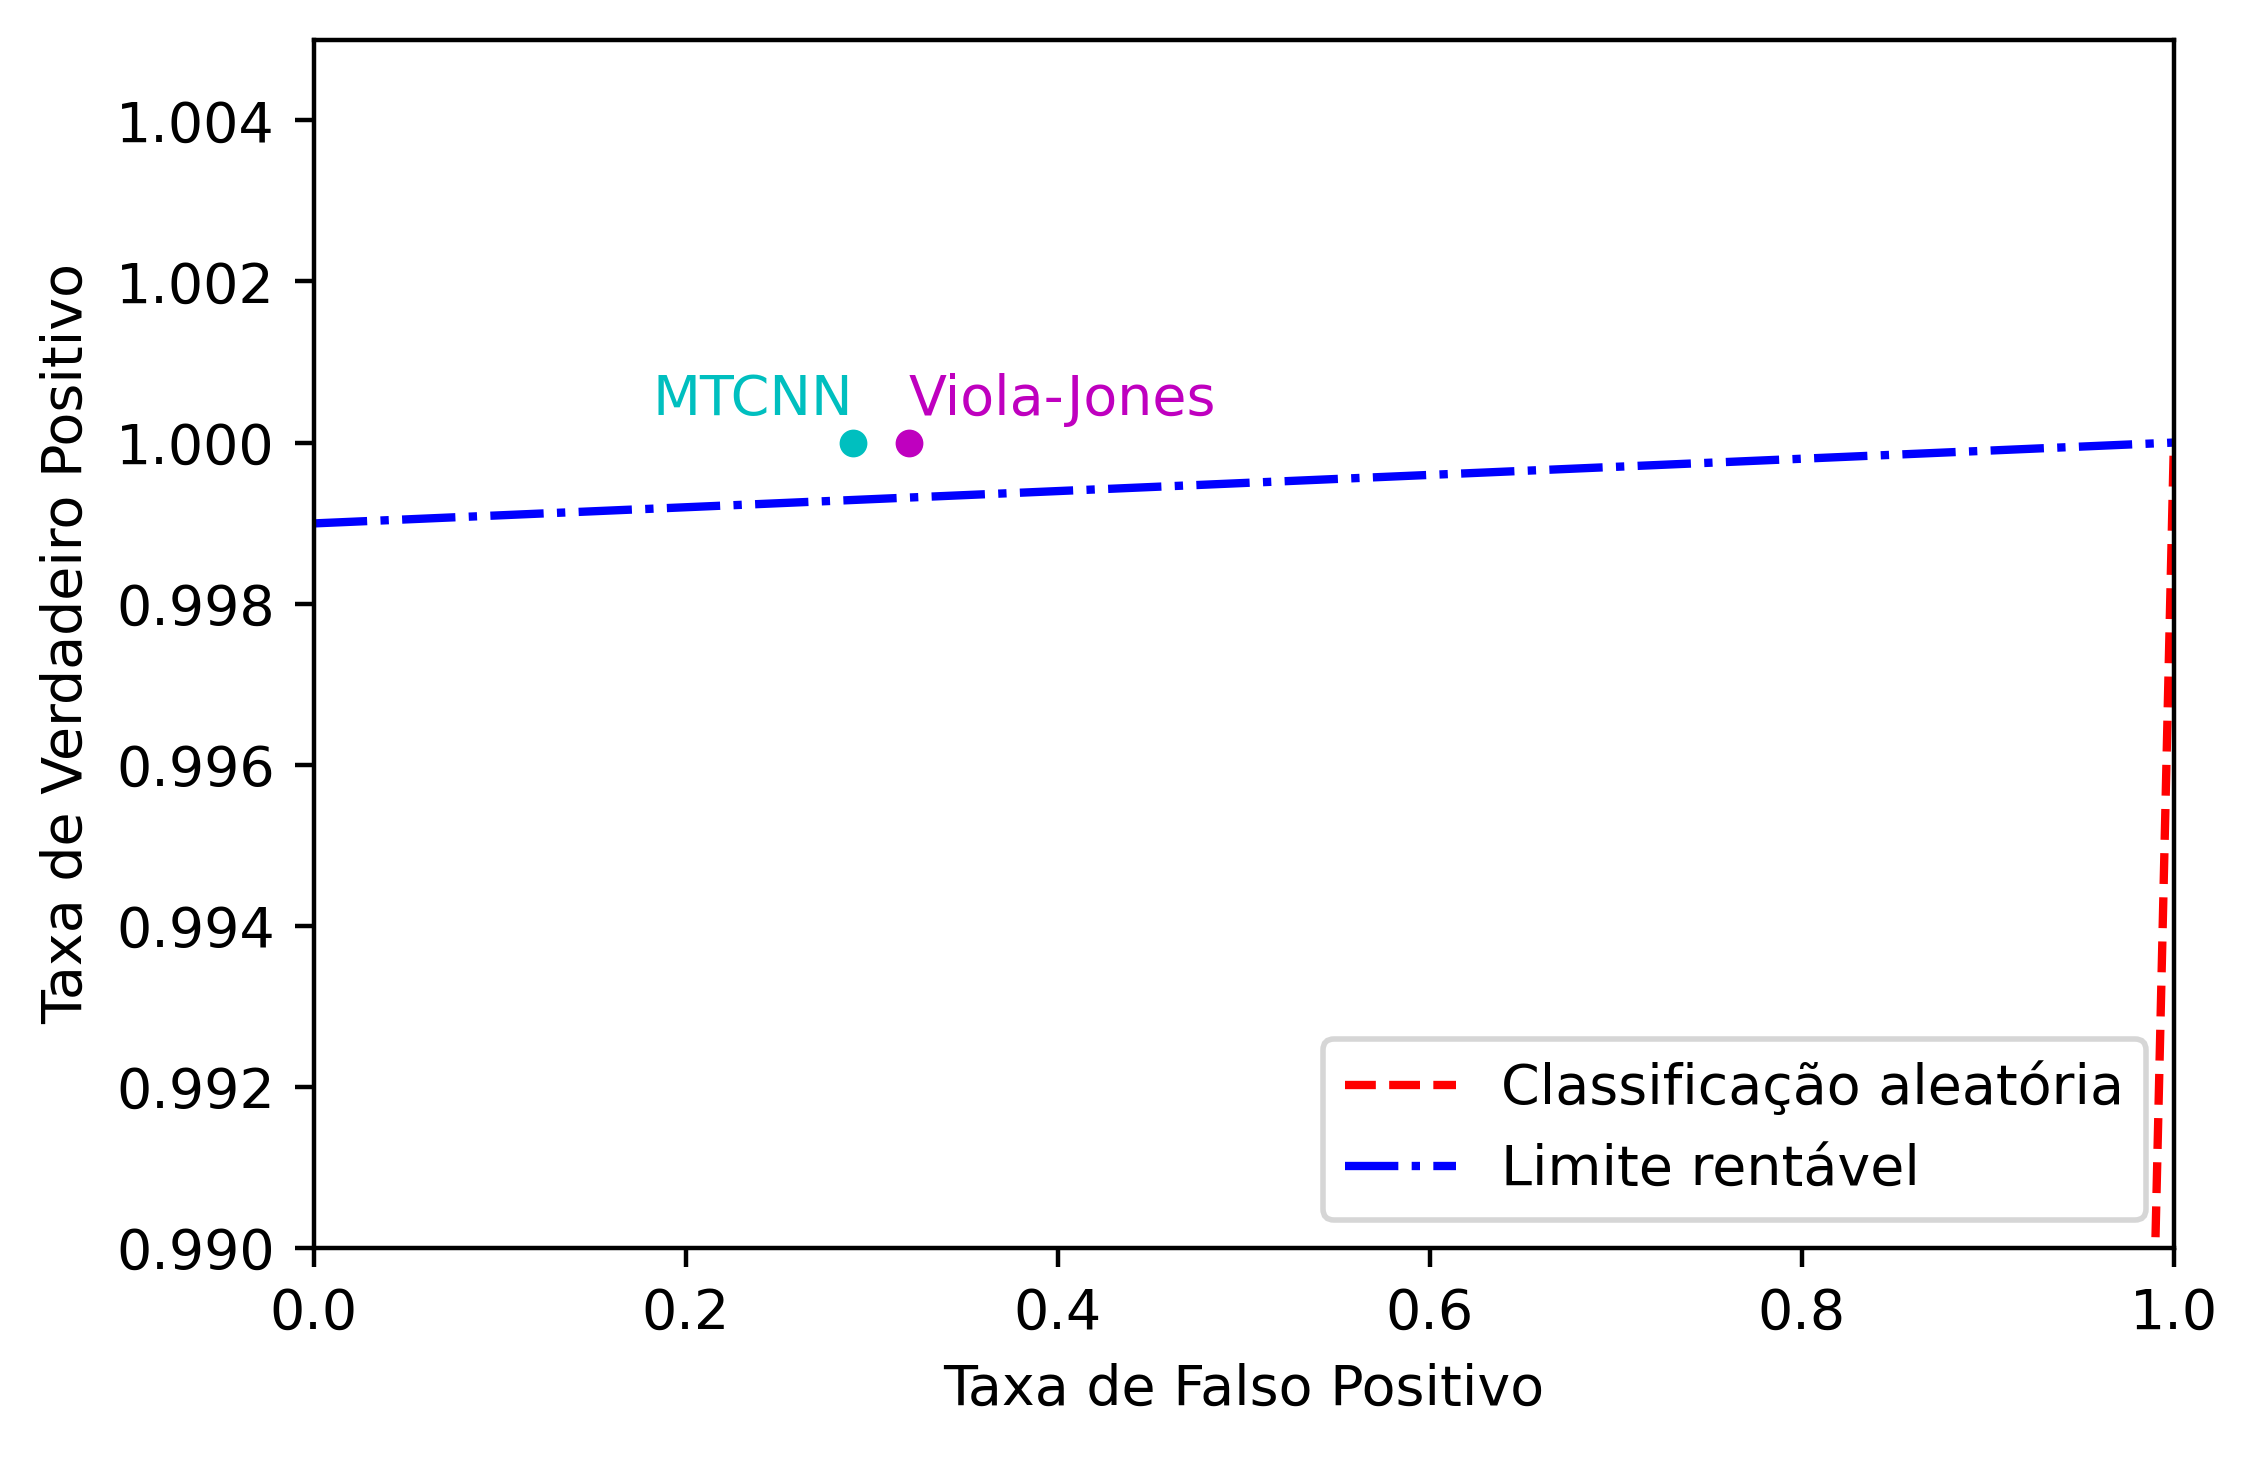
\includegraphics[scale=1]{figs/curva_roc_results_mtcnn.png}
    \legend{Fonte: Própria (2020)}
    \label{fig:results_roc_mtcnn}
\end{figure}

\begin{table}[htbp]
    \caption{Resultado do método MTCNN e melhor resultado do método de Viola-Jones.}
    \label{tab:results_mtcnn}
    \centering
    \renewcommand{\arraystretch}{1.4}
    \begin{tabular}{lrrrrrr}
        \hline\hline
        Método      & FE   & MV & sensibilidade & Especificidade & Acurácia & Lucro\footnote{Lucro refere-se ao lucro obtido por imagem analisada.} \\
        \midrule
        MTCNN       & -    & -  & 100,00\%      & 71,00\%        & 94,20\%  & R\$ 0,142                                                             \\
        Viola-Jones & 1,10 & 4  & 100,00\%      & 68,00\%        & 93,60\%  & R\$ 0,136                                                             \\
        \hline\hline
    \end{tabular}
\end{table}

Analisando os resultados de sensibilidade, especificidade e acurácia de cada um dos classificadores na Tabela \ref{tab:results_identify} e da Tabela \ref{tab:results_mtcnn}, a matriz de confusão do resultado que mais lucrativo utilizando o método de Viola-Jones na Tabela \ref{tab:matriz_de_confusao_viola} e a matriz de confusão do resultado utlizando o método MTCNN na Tabela \ref{tab:matriz_de_confusao_mtcnn}, é possível obter algumas conclusões interessantes.

\begin{table}[htbp]
    \caption{Matriz de confusão para o resultado mais lucrativo do método de Viola-Jones.}
    \label{tab:matriz_de_confusao_viola}
    \centering
    \renewcommand{\arraystretch}{1.4}
    \begin{tabular}{c|cc|c}\hline\hline
                       & \textit{B} & $\overline{B}$ & Soma  \\
        \hline
        \textit{A}     & 80.0\%     & 00.0\%         & 80\%  \\
        $\overline{A}$ & 06.4\%     & 13.6\%         & 20\%  \\
        \hline
        Soma           & 86.4\%     & 13.6\%         & 100\% \\
        \hline\hline
    \end{tabular}
\end{table}

\begin{table}[htbp]
    \caption{Matriz de confusão para o resultado do método de MTCNN.}
    \label{tab:matriz_de_confusao_mtcnn}
    \centering
    \renewcommand{\arraystretch}{1.4}
    \begin{tabular}{c|cc|c}\hline\hline
                       & \textit{B} & $\overline{B}$ & Soma  \\
        \hline
        \textit{A}     & 80.0\%     & 00.0\%         & 80\%  \\
        $\overline{A}$ & 05.8\%     & 14.2\%         & 20\%  \\
        \hline
        Soma           & 85.8\%     & 14.2\%         & 100\% \\
        \hline\hline
    \end{tabular}
\end{table}

Comparando tal resultado com a análise da equação que define o limiar lucrativo da classificação, é possível perceber que cada imagem positiva que é classificada como negativa gera um prejuízo muito elevado, que precisa ser compensado com a classificação correta de uma grande quantidade de imagens negativas. Para o classificador estudado, percebe-se que todos os cenários lucrativos apresentam sensibilidade igual a 100\%, ou seja, todas imagens positivas foram classificadas corretamente.

É curioso notar que o lucro não é diretamente proporcional a acurácia do detector, destacando que a configuração de maior acurácia (94,60\%), com fator de escala igual a 1,25 e número mínimo de vizinhos igual a 6, apresentou prejuízo de R\$ 4,814 por imagem, tal fato também ocorre devido ao prejuízo elevado de classificar uma imagem positiva de forma incorreta.
